The next prototype, Tritium-IFIC 1, was intended to overcome the problems and limitations found in the previous prototype, section \ref{subsec:TritiumIFIC0}. To do so, some improvements were applied on it:

\begin{enumerate}

\item{} First, as we said before, the fiber bundle is arranged straight to optimize the photon collection efficiency of the fibers.

\item{} Second, a special fiber cleaning protocol, previously explained in section \ref{subsubsec:CleaningProcess}, was applied on the fibers. It was used to improve the interfaces between fiber and tritiated water, creating a better wetting property of the fiber, which will result in more tritium events detected and a greater photon collection efficiency.

\item{} Lastly, as we have seen in our previous fiber characterization study, shown in section \ref{subsubsec:CharacterizationFibers}, the photon collection efficiency of the fibers used is poor, so a large number of photons will be lost in each tritium event.

It is an innerent characteristic of the fiber which we cannot change but, to reduce its effect, we will use a Teflon vessel for Tritium prototypes.

Teflon is an interesting material for its optical properties, specifically its reflection factor, which is very close to $100\%$ at the working wavelength. It means that practically all the photons that reach the walls of the vessel will be reflected back to the fiber.

\end{enumerate}

Taking into accout all this modification, the following prototype was designed, built and tested, whose name is Tritium-IFIC 1. It consists of 64 scintillating fibers, with a length of $20~\cm$, which are arranged in a straight position using a teflon structure, shown in figure \ref{fig:TeflonStructureFibersTritiumIFIC1}, in which these fibers are fixed in an $8\cdot{}8$ square matrix.

\begin{figure}[h]
\centering
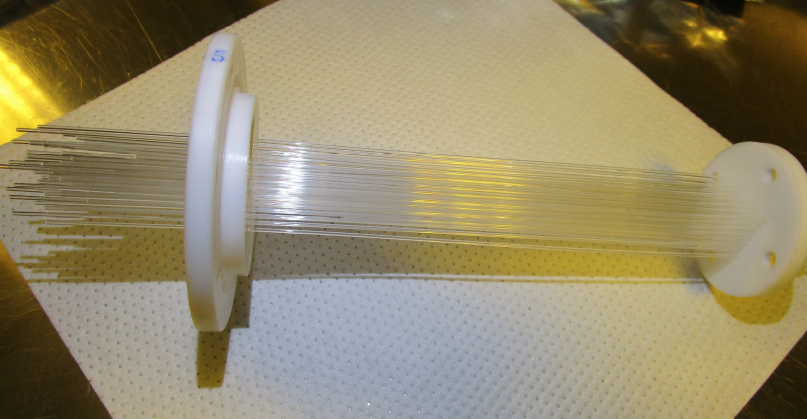
\includegraphics[scale=0.4]{5Prototypes/52PreliminarPrototypes/522TritiumIFIC1/FiberMatrixTeflonStructure.png}
\caption{Teflon structure used to arrange the fibers of Tritium-IFIC 1 prototype in a matrix of $8\cdot{}8$.\label{fig:TeflonStructureFibersTritiumIFIC1}}
\end{figure}

A new teflon vessel was designed and built, shown in figure \ref{fig:TeflonVesselTritumIFIC1}. It has a cylindrical hole whose internal diameter and length are $48~\mm$ and $200~\mm$ respectively, where the fiber structure will be placed. 

\begin{figure}[h]
 \centering
  \subfloat[]{
   \label{subfig:TeflonVesselTritumIFIC1a}
    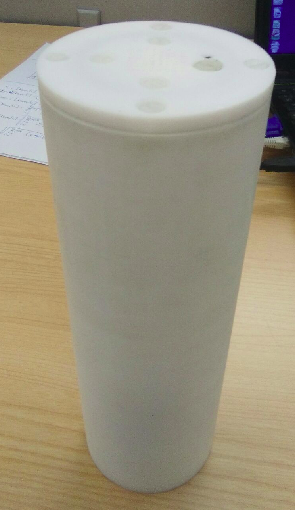
\includegraphics[angle=0, width=0.30\textwidth]{5Prototypes/52PreliminarPrototypes/522TritiumIFIC1/TeflonVesselTritiumIFIC1a.png}}
    %\newline
  \subfloat[]{
   \label{subfig:TeflonVesselTritumIFIC1b}
    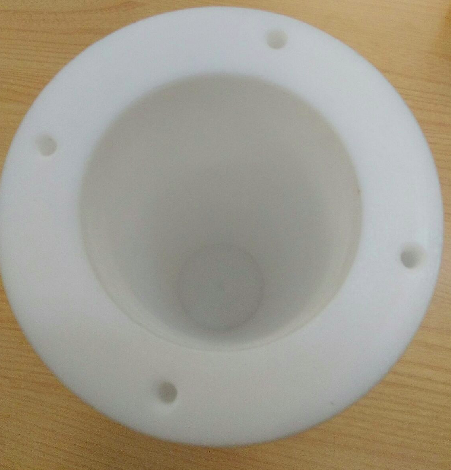
\includegraphics[angle=0, width=0.45\textwidth]{5Prototypes/52PreliminarPrototypes/522TritiumIFIC1/TeflonVesselTritiumIFIC1b.png}}
 \caption{Teflon vessel of Tritium-IFIC 1 prototype}
 \label{fig:TeflonVesselTritumIFIC1}
\end{figure}

In addition to cutting and polishing the scintillating fibers used, a cleaning process, described in section \ref{subsubsec:CleaningProcess}, was applied to them to achieve a better tritium water-fiber interface.

A general view of this prototype is shown in figure \ref{fig:TritumIFIC1}, which, for radioactivity safety reasons, will be read using only one PMT.

\begin{figure}[h]
 \centering
  \subfloat[]{
   \label{subfig:TritumIFIC1a}
    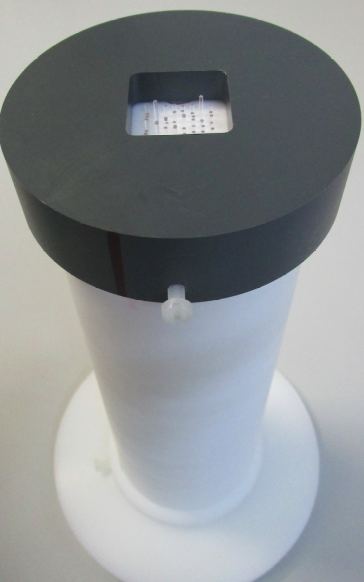
\includegraphics[angle=0, width=0.40\textwidth]{5Prototypes/52PreliminarPrototypes/522TritiumIFIC1/TritiumIFIC1a.png}}
    %\newline
  \subfloat[]{
   \label{subfig:TritumIFIC1b}
    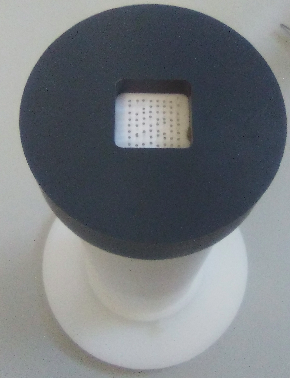
\includegraphics[angle=0, width=0.4\textwidth]{5Prototypes/52PreliminarPrototypes/522TritiumIFIC1/TritiumIFIC1b.png}}
 \caption{A general view of Tritium-IFIC 1 prototype}
 \label{fig:TritumIFIC1}
\end{figure}

The PMT used was the model R8520-460, from Hamamatsu Photonics company \cite{DataSheetPMTs} and it was coupled directly to the fiber bundle using optical grease \cite{OpticalGrease}. It was powered at $-800~\volt$, at which, its quantum efficiency is $28\%$.

The signal from this PMT was processed and analyzed using the same electronic configuration as that used for the Tritium-IFIC 0 prototype.

Unlike the previous prototype, only one Tritium-IFIC 1 was built. First, it was filled with ultrapure water ($118~\milli\liter$, uncertainty of $0.05\%$) and several background measurements were taken over a week. Then, it was emptied and refilled using $118~\milli\liter$ (uncertainty of $0.05\%$) of the radioactive liquid source of tritium explained in appendix \ref{App:TritiumSourcePreparation}.

The result of this measurement is shown in the section \ref{subsec:ResultsTritiumIFIC1}, where it will be discussed and compared with the result obtained with the previous prototype, Tritium-IFIC 0.